\scanpage{23}
\mspage{11}
\margin{22}

une des extrémités serait un sommet de $\Sigma$, comme

\figure{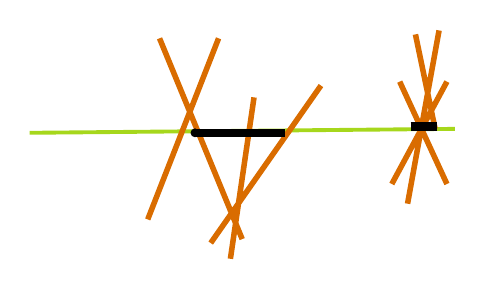
\begin{tikzpicture}[x=1cm,y=1cm]
\draw[yellow!65!green,line width=1.4pt] (-2.2,0)--(3.2,.05);
\draw[orange!85!black,line width=2pt] (-.7,-1.1)--(.2,1.2) (.5,-1.35)--(-.55,1.2) (.35,-1.6)--(.65,.45) (.1,-1.4)--(1.5,.6) (2.4,-.65)--(3.1,.65) (3.1,-.65)--(2.5,.65) (2.6,-.9)--(3,1.3) (2.95,.05)--(2.7,1.25);
\draw[black,line width=3pt] (-.1,0)--(1.04,0) (2.64,.08)--(2.97,.08);
\fill(-.1,0)circle(1.6pt);
\end{tikzpicture}}

(on lui fait correspondre une arête libre de $\Gamma(\underline\Sigma)$, sans autre sommet au bout); \uline{il serait pratique} d'inclure, comme dit plus haut, les antipodiques de \inserted{ts} ces arcs (de spécialisation, ou de pseudo-spécialisation --- pour un arc de vraie spécialisation, \deleted{\unsure{il en est}} l'antipodique est \unsure{soit} de spécialisation, soit de pseudo-spécialisation) --- également en bouts libres. Soit $\operatorname{Pol}^*(D)$ ce polygône (plus grand que celui précédemment désigné sous ce vocable). On trouve alors un \deleted{\unsure{bon}} iso de $\operatorname{Pol}^*(D)$ avec un \uline{sous-polygône} de $\operatorname{Pol}^*(D')$, mais ce n'est pas néc. un iso, car de nouveaux arcs de pseudo-spécialisation \inserted{(ou triangles)} $t$ peuvent être créés par spécialisation, dans le cas où l'une ou l'autre des deux faces adjacentes au triangle $T$ sur l'une de ses \unsure{deux} faces latérales est un carré. Donc \unsure{il peut alors y avoir} deux \inserted{\unsure{voisins de}} sommets \inserted{\unsure{contigus}} dans l'image de

\figure{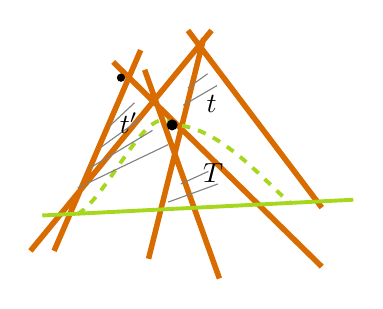
\begin{tikzpicture}[x=1cm,y=1cm]
\coordinate(A)at(0,1.1);\coordinate(B)at(-.65,1.7);\coordinate(C)at(.35,2.05);
\draw[orange!85!black,line width=2pt] (-1.8,-.5)--(.5,2.3) (-1.5,-.5)--(-.4,2.05) (-.75,1.9)--(1.9,-.7) (-.3,-.6)--(.4,2.2) (.6,-.85)--(-.35,1.8) (.2,2.3)--(1.9,.05);
\draw[yellow!65!green,line width=1.4pt] (-1.65,-.05)--(2.3,.15);
\draw[yellow!65!green,line width=1.4pt,dashed] (-1.2,-.03)..controls(-.8,.2)and(-.3,1.45)..(0,1.1)..controls(.6,1.1)and(1.2,.35)..(1.5,.11);
\draw[gray] (-1.2,.3)--(-.05,.85) (-1.05,.55)--(-.25,1.03) (-.9,.82)--(-.4,1.18) (-.8,1.08)--(-.48,1.38) (.14,1.35)--(.57,1.6) (.2,1.57)--(.45,1.75) (.11,.35)--(.46,.51) (-.05,.12)--(.58,.35);
\fill(A)circle(2pt);\fill(B)circle(1.5pt);
\node at(-.55,1.12){$t'$};\node at(.5,1.37){$t$};\node at(.52,.49){$T$};
\end{tikzpicture}}

\figure{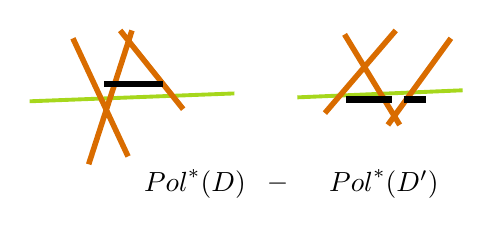
\begin{tikzpicture}[x=1cm,y=1cm]
\draw[yellow!65!green,line width=1.4pt] (-1.1,0)--(1.5,.1) (2.3,.05)--(4.4,.14);
\draw[orange!85!black,line width=2pt] (-.35,-.8)--(.2,.9) (.15,-.7)--(-.55,.8) (.05,.9)--(.85,-.1) (2.65,-.15)--(3.55,.9) (3.6,-.3)--(2.9,.85) (3.45,-.3)--(4.25,.8);
\draw[black,line width=2.5pt] (-.15,.22)--(.6,.22) (2.92,.02)--(3.5,.02) (3.65,.02)--(3.94,.02);
\node at(1,-1.05){$\operatorname{Pol}^*(D)$};\node at(2.05,-1.05){$-$};\node at(3.4,-1.05){$\operatorname{Pol}^*(D')$};
\end{tikzpicture}}

\margin{\uline{NB} la pondération du polygône $\operatorname{Pol}^*(D)$ est stable par antipodie.}

L'introduction de $\operatorname{Pol}^*(D)$ est intéressante, puisqu'elle est stable par antipodisme. Si on veut exprimer la compatibilité avec les pondérations, on dira que deux \deleted{arêtes} \inserted{sommets} qui se correspondent ont $=$ pondérations, ainsi que deux arêtes qui se correspondent. Quand $\operatorname{Pol}^*(D)\mathbin{-}\operatorname{Pol}^*(D')$ n'est pas un iso, alors il y a \deleted{les} un ou deux des sommets adjacents \deleted{aux} aux sommets $(D',a)$, $(D',a')$ de $\operatorname{Pol}^*(D')$ qui manquent.

\margin{\uline{NB} La pondération d'une \uline{arête} de $\operatorname{Pol}^*(D)$ peut être nulle --- \deleted{p.ex} entre \deleted{\unsure{deux adjacents}} \inserted{un} arc de \deleted{spécialisation} générisation, \unsure{et} un arc de ps.-spéc. adjacent cf figure ci dessus et aussi entre l'antip. d'un arc de spéc et un autre arc de spécialisation.}
